% Channel-reliance figure (data: 04_Stage4_Evidence.md multi-seed zero-out table).
\begin{figure}[t]
  \centering
  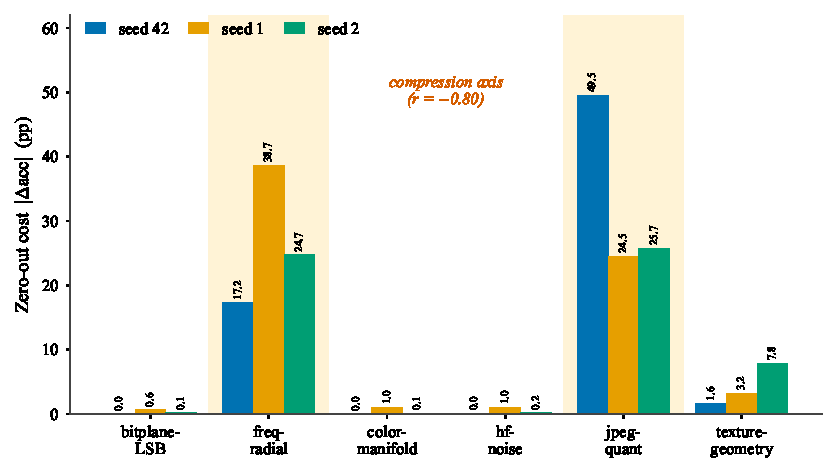
\includegraphics[width=\textwidth]{figs/fig_channel_reliance.pdf}
  \caption{\textbf{Causal channel reliance is concentrated on a compression axis, across
    three seeds.} Accuracy drop (pp) from zeroing each bottleneck channel, mean over the
    seven evaluation generators, for seeds 42/1/2. In every seed the two tall bars are the
    correlated compression pair \texttt{freq-radial} and \texttt{jpeg-quant} (shaded;
    $r{=}{-}0.80$), which dwarf the other four channels (all $|\Delta|<3.3$\,pp). Which
    member of the pair carries the larger drop \emph{shifts} across seeds (seed-42:
    \texttt{jpeg-quant}; seed-1: \texttt{freq-radial}; seed-2: nearly tied): the compression
    \emph{axis} is stable, the named \emph{carrier} is not. The linear-head weights do not
    reveal this ordering; only causal ablation does (\S{}4.3a).}
  \label{fig:reliance}
\end{figure}
